\documentclass[tikz,convert={outfile=\jobname.svg}]{standalone}
\newcommand{\Esc}{\framebox{\texttt{Esc}}}
\newcommand{\Enter}{\framebox{\texttt{Enter}}}
\usetikzlibrary{positioning,automata}
\tikzset{ %inner sep = 0.5mm,
  %minimum size = 5mm,
  >=latex,
  every state/.style={draw=blue!50,thick,fill=blue!20,minimum size=1.8cm},
  {small point/.style} ={circle,draw=blue!60,fill=blue!30,inner sep=0, minimum size= 1mm},
  box/.style ={circle,draw=black!60,fill=black!20,inner
  sep=5pt,fill=blue!30,draw=blue!60,rectangle},
  {edge/.style} ={thick,draw},
  {dedge/.style} ={draw,->},
 }
\begin{document}
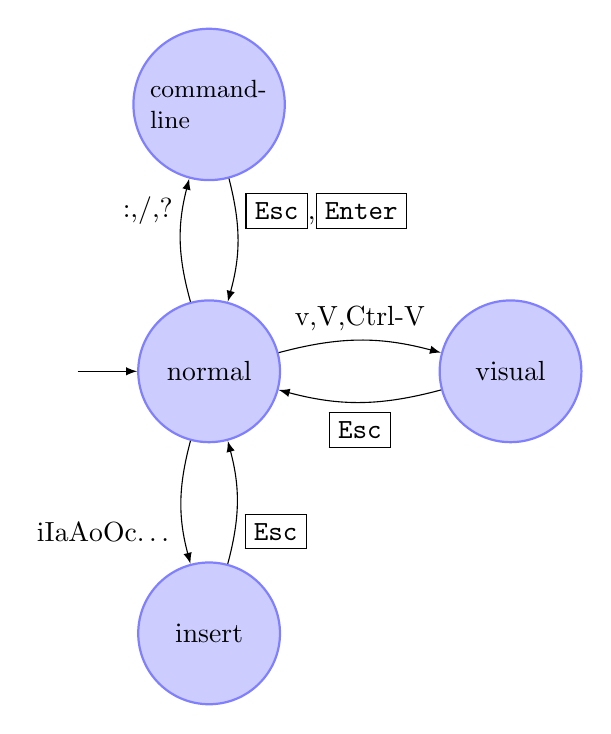
\begin{tikzpicture}[node distance=1.5cm,/tikz/initial text=,
                initial distance=5ex]
        \node[state,initial] (n) at (0,0) {normal}; 
        \node[state] (c) [above=of n]
                {\parbox[c]{1.5cm}{\small command-line}}; 
        \node[state] (v) [right=2cm of n] {visual}; 
        \node[state] (i) [below=1.5cm of n] {insert}; 
        %\node (h) [below=.5cm of i] {:help vim-modes}; 
        \path[dedge] (n) edge[bend left=15] node[left,near end] {:,/,?} (c)
                edge[bend left=15] node[above] {v,V,Ctrl-V} (v)
                edge[bend right=15] node[left,near end] {iIaAoOc\ldots} (i);
        %\path[dedge] (-1.5cm,0) -- (n);
        \path[dedge] (i) edge[bend right=15] node[right,near start] {\Esc} (n);
        \path[dedge] (v) edge[bend left=15] node[below] {\Esc} (n);
        \path[dedge] (c) edge[bend left=15] node[right,near start]
        {\Esc,\Enter} (n);
\end{tikzpicture}
\end{document}
